\section{An Introduction to Vectors}\label{sec:vector_intro}

Many quantities we think about daily can be described by a single number: temperature, speed, cost, weight and height. There are also many other concepts we encounter daily that cannot be described with just one number. For instance, a weather forecaster often describes wind with its speed and its direction (``\ldots with winds from the southeast gusting up to 30 mph \ldots''). When applying a force, we are concerned with both the magnitude and direction of that force. In both of these examples, \emph{direction} is important. Because of this, we study \emph{vectors}, mathematical objects that convey both magnitude and direction information.\bigskip

One ``bare-bones'' definition of a vector is based on what we wrote above: ``a vector is a mathematical object characterized by its magnitude and direction.'' This definition leaves much to be desired, as it gives no indication as to how such an object is to be used. Several other definitions exist; we choose here a definition rooted in a geometric visualization of vectors. It is very simplistic but readily permits further investigation.

\mtable{Drawing the same vector with different initial points.}{fig:vectintro1}{\pdftooltip{\begin{tikzpicture}
\begin{axis}[width=1.16\marginparwidth,tick label style={font=\scriptsize},
axis y line=middle,axis x line=middle,name=myplot,axis on top,
ymin=-5.5,ymax=5.5,xmin=-5.5,xmax=5.5]
\draw[very thick,->,>=stealth] (axis cs:0,0) --(axis cs:3,1);
\draw[very thick,->,>=stealth] (axis cs:-2,-3) --(axis cs:1,-2);
\draw[very thick,->,>=stealth] (axis cs:-4,1) --(axis cs:-1,2);
\draw[very thick,->,>=stealth] (axis cs:2,-4) --(axis cs:5,-3);
\end{axis}
\node [right] at (myplot.right of origin) {\scriptsize $x$};
\node [above] at (myplot.above origin) {\scriptsize $y$};
\end{tikzpicture}}{ALT-TEXT-TO-BE-DETERMINED}}

\begin{definition}[Vector]\label{def:vector}
A \textbf{vector} is a directed line segment.\bigskip

Given points $P$ and $Q$ (either in the plane or in space), we denote with $\vv{PQ}$ the vector \emph{from $P$ to $Q$}. The point $P$ is said to be the \textbf{initial point} of the vector, and the point $Q$ is the \textbf{terminal point}. \bigskip

The \textbf{magnitude}, \textbf{length} or \textbf{norm} of $\vv{PQ}$ is the length of the line segment $\overline{PQ}$: $\norm{\vv{PQ}} = \norm{\overline{PQ}}$.\bigskip

Two vectors are \textbf{equal} if they have the same magnitude and direction.
\index{vectors}\index{vectors!definition}\index{vectors!norm}
\index{vectors!magnitude}\index{norm}\index{magnitude of vector}
\index{terminal point}\index{initial point}
\end{definition}

\mnote{\textbf{Note:} Instead of $\norm{\vv{PQ}}$, some texts use $\abs{\vv{PQ}}$ and rely on context to know if it is the norm of a vector or the absolute value of a scalar.}

\autoref{fig:vectintro1} shows multiple instances of the same vector. Each directed line segment has the same direction and length (magnitude), hence each is the same vector.

%Given two points $P$ and $Q$ (either in the plane or in space), the line segment that starts at $P$ and ends at $Q$ is a vector, denoted $\vv{PQ}$. The point $P$ is said to be the \textbf{initial} point of the vector, and the point $Q$ is the \textbf{terminal point}. We define the magnitude of $\vv{PQ}$ as the length of the line segment $\overline{PQ}$: $\norm{\vv{PQ}}=\norm{\overline{PQ}}$.

We use $\mathbb{R}^2$ (pronounced ``r two'') to represent all the vectors in the plane, and use $\mathbb{R}^3$ (pronounced ``r three'') to represent all the vectors in space.\index{r2@$\mathbb{R}^2$}\index{r3@$\mathbb{R}^3$}
We use the word ``scalar'' to refer to a real number that is not a vector.\index{scalar}

\mtable{Illustrating how equal vectors have the same displacement.}{fig:vectintro2}{\pdftooltip{\begin{tikzpicture}
\begin{axis}[width=1.16\marginparwidth,tick label style={font=\scriptsize},
axis y line=middle,axis x line=middle,name=myplot,axis on top,minor x tick num=1,
minor y tick num=1,ymin=-4.5,ymax=4.5,xmin=-4.5,xmax=4.5]
\draw[very thick,->,>=stealth] (axis cs:1,0) node [above] {\scriptsize $P$}
 --(axis cs:3,1)node [above] {\scriptsize $Q$};
\draw[very thick,->,>=stealth] (axis cs:-3,1)node [above] {\scriptsize $R$}
 --(axis cs:-1,2)node [above] {\scriptsize $S$};
\end{axis}
\node [right] at (myplot.right of origin) {\scriptsize $x$};
\node [above] at (myplot.above origin) {\scriptsize $y$};
\end{tikzpicture}}{ALT-TEXT-TO-BE-DETERMINED}}

Consider the vectors $\vv{PQ}$ and $\vv{RS}$ as shown in \autoref{fig:vectintro2}. The vectors look to be equal; that is, they seem to have the same length and direction. Indeed, they are. Both vectors move 2 units to the right and 1 unit up from the initial point to reach the terminal point. One can analyze this movement to measure the magnitude of the vector, and the movement itself gives direction information (one could also measure the slope of the line passing through $P$ and $Q$ or $R$ and $S$). Since they have the same length and direction, these two vectors are equal.

This demonstrates that inherently all we care about is \emph{displacement}; that is, how far in the $x$, $y$ and possibly $z$ directions the terminal point is from the initial point. Both the vectors $\vv{PQ}$ and $\vv{RS}$ in \autoref{fig:vectintro2} have an $x$-displacement of 2 and a $y$-displacement of 1. This suggests a standard way of describing vectors in the plane. A vector whose $x$-displacement is $a$ and whose $y$-displacement is $b$ will have terminal point $(a,b)$ when the initial point is the origin, $(0,0)$. This leads us to a definition of a standard and concise way of referring to vectors.

\begin{definition}[Component Form of a Vector]\label{def:vector_component}
\mbox{}\\[-2\baselineskip]\parbox[t]{\linewidth}{\begin{enumerate}
	\item The \textbf{component form} of a vector $\vec{v}$ in $\mathbb{R}^2$, whose terminal point is $(a,b)$ when its initial point is $(0,0)$, is $\bracket{a,b}.$ 
	
	\item The \textbf{component form} of a vector $\vec{v}$ in $\mathbb{R}^3$, whose terminal point is $(a,b,c)$ when its initial point is $(0,0,0)$, is $\bracket{a,b,c}.$ 
	
	%The component form of the vector $\vv{PQ}$, where $P=(x_1,y_1,z_1)$ and $Q=(x_2,y_2,z_2)$ is 
	%\[\vv{PQ} =\bracket{x_2-x_1, y_2-y_1,z_2-z_1}.\]
\end{enumerate}}
The numbers $a$, $b$ (and $c$, respectively) are the \textbf{components} of $\vec v$.
\index{vectors!component form}
\end{definition}

\mnote{\textbf{Note:} Instead of $\vec{v}$, some texts use boldface: $\mathbf{v}$. The advantage of $\mathbf{v}$ is that it tends to be easier to read.  The advantage of $\vec{v}$ is that it's easier to write.}

It follows from the definition that the component form of the vector $\vv{PQ}$, where $P=(x_1,y_1)$ and $Q=(x_2,y_2)$ is
\[\vv{PQ} =\bracket{x_2-x_1, y_2-y_1};\]
in space, where $P=(x_1,y_1,z_1)$ and $Q=(x_2,y_2,z_2)$, the component form of $\vv{PQ}$ is	\[\vv{PQ} =\bracket{x_2-x_1, y_2-y_1,z_2-z_1}.\]

\youtubeVideo{60btq9PN8IM}{An Introduction to Vectors, Part 1}

We practice using this notation in the following example.

\begin{example}[Using component form notation for vectors]\label{ex_vect1}
\mbox{}\\[-2\baselineskip]\parbox[t]{\linewidth}{%
\begin{enumerate}
	\item	Sketch the vector $\vec v=\bracket{2,-1}$ starting at $P=(3,2)$ and find its magnitude.
	\item	Find the component form of the vector $\vec w$ whose initial point is $R=(-3,-2)$ and whose terminal point is $S=(-1,2)$.
	\item	Sketch the vector $\vec u =\bracket{2,-1,3}$ starting at the point $Q = (1,1,1)$ and find its
magnitude.
\end{enumerate}}\vspace{0pt}
\solution
\begin{enumerate}
	\item Using $P$ as the initial point, we move 2 units in the positive $x$-direction and $-1$ units in the positive $y$-direction to arrive at the terminal point $P\,'=(5,1)$, as drawn in \autoref{fig:vect1}(a).
	
	The magnitude of $\vec v$ is determined directly from the component form:
	\[\norm{\vec v} =\sqrt{2^2+(-1)^2} = \sqrt{5}.\]
	\mtable{Graphing vectors in \autoref{ex_vect1}.}{fig:vect1}{%
\pdftooltip{\begin{tikzpicture}
\begin{axis}[width=1.16\marginparwidth,tick label style={font=\scriptsize},
axis y line=middle,axis x line=middle,name=myplot,axis on top,minor x tick num=4,
minor y tick num=4,ymin=-5.5,ymax=5.5,xmin=-5.5,xmax=5.9]
\draw[very thick,->,>=stealth] (axis cs:3,2) node [left] {\scriptsize $P$}
--(axis cs:5,1)node [shift={(5pt,0pt)}] {\scriptsize $P\,'$};
\draw[very thick,->,>=stealth] (axis cs:-3,-2)node [below left] {\scriptsize $R$}
 --(axis cs:-1,2)node [above] {\scriptsize $S$};
\end{axis}
\node [right] at (myplot.right of origin) {\scriptsize $x$};
\node [above] at (myplot.above origin) {\scriptsize $y$};
\end{tikzpicture}}{ALT-TEXT-TO-BE-DETERMINED}
	\\(a)\\[20pt]
	\myincludeasythree{width=\marginparwidth,
3Droll=0,
3Dortho=0.004,
3Dc2c=.3 .9 .3,
3Dcoo=49 42 58,
3Droo=150}{width=\marginparwidth}{figures/figvectintro3b_3D}\\
	(b)}
	
	\item	Using the paragraph following \autoref{def:vector_component}, we have
	\[\vv{RS} =\bracket{-1-(-3), 2-(-2)}=\bracket{2,4}.\]
	One can readily see from \autoref{fig:vect1}(a) that the $x$- and $y$-displacement of $\vv{RS}$ is 2 and 4, respectively, as the component form suggests.
	
	\item	Using $Q$ as the initial point, we move 2 units in the positive $x$-direction, $-1$ unit in the positive $y$-direction, and 3 units in the positive $z$-direction to arrive at the terminal point $Q' = (3,0,4)$, illustrated in \autoref{fig:vect1}(b).
	
	The magnitude of $\vec u$ is:
	\[\norm{\vec u} = \sqrt{2^2+(-1)^2+3^2} = \sqrt{14}.\]
\end{enumerate}
\end{example}

Now that we have defined vectors, and have created a nice notation by which to describe them, we start considering how vectors interact with each other. That is, we define an \emph{algebra} on vectors.

\begin{definition}[Vector Algebra]\label{def:vector_algebra}
\index{vectors!algebra of}\mbox{}\\[-2\baselineskip]\parbox[t]{\linewidth}{\begin{enumerate}
	\item Let $\vec u =\bracket{u_1,u_2}$ and $\vec v =\bracket{v_1,v_2}$ be vectors in $\mathbb{R}^2$, and let $c$ be a scalar.
		\begin{enumerate}
			\item The addition, or sum, of the vectors $\vec u$ and $\vec v$ is the vector
			\[\vec u+\vec v =\bracket{u_1+v_1, u_2+v_2}.\]
			\item	The product of $c$ and $\vec v$ is the vector 
			\[c\vec v = c\bracket{v_1,v_2}=\bracket{cv_1,cv_2}.\]
		\end{enumerate}
	\item Let $\vec u =\bracket{u_1,u_2,u_3}$ and $\vec v =\bracket{v_1,v_2,v_3}$ be vectors in $\mathbb{R}^3$, and let $c$ be a scalar. 
		\begin{enumerate}
			\item The addition, or sum, of the vectors $\vec u$ and $\vec v$ is the vector
			\[\vec u+\vec v =\bracket{u_1+v_1, u_2+v_2, u_3+v_3}.\]
			\item	The product of $c$ and $\vec v$ is the vector 
			\[c\vec v = c\bracket{v_1,v_2,v_3}=\bracket{cv_1,cv_2,cv_3}.\]
		\end{enumerate}
\end{enumerate}}
\end{definition}

In short, we say addition and multiplication are computed ``componentwise.''  We also define vector subtraction using these two operations:
%It follows from the properties of the real numbers and \autoref{def:vector_algebra} that
\[\vec u-\vec v = \vec u + (-1)\vec v.\]

\begin{example}[Adding vectors]\label{ex_vect2}
Sketch the vectors $\vec u =\bracket{1,3}$, $\vec v =\bracket{2,1}$ and $\vec u+\vec v$ all with initial point at the origin.
\solution
We first compute $\vec u +\vec v$.
%
\mtable{Graphing the sum of vectors in \autoref{ex_vect2}.}{fig:vect2}{\pdftooltip{\begin{tikzpicture}
\begin{axis}[width=1.16\marginparwidth,tick label style={font=\scriptsize},
axis y line=middle,axis x line=middle,name=myplot,axis on top,minor x tick num=1,
minor y tick num=1,ymin=-.5,ymax=4.1,xmin=-.5,xmax=4.1]
\draw[very thick,->,>=stealth] (axis cs:0,0) --(axis cs:1,3)
 node [pos=.5,above,rotate=70] {\scriptsize $\vec u$};
\draw[very thick,->,>=stealth] (axis cs:0,0) --(axis cs:2,1)
 node [pos=.5,above,rotate=40] {\scriptsize $\vec v$};
\draw[very thick,->,>=stealth] (axis cs:0,0) --(axis cs:3,4)
 node [pos=.5,above,rotate=50] {\scriptsize $\vec u+\vec v$};
\end{axis}
\node [right] at (myplot.right of origin) {\scriptsize $x$};
\node [above] at (myplot.above origin) {\scriptsize $y$};
\end{tikzpicture}}{ALT-TEXT-TO-BE-DETERMINED}}
%
\begin{align*}
	\vec u+\vec v &=\bracket{1,3}+\bracket{2,1}\\
	&=\bracket{3,4}.
\end{align*}
These are all sketched in \autoref{fig:vect2}.
\end{example}

As vectors convey magnitude and direction information, the sum of vectors also convey length and magnitude information. Adding $\vec u+\vec v$ suggests the following idea:
\begin{quotation}
``Starting at an initial point, go out $\vec u$, then go out $\vec v$.''
\end{quotation}

This idea is sketched in \autoref{fig:vect2b}, where the initial point of $\vec v$ is the terminal point of $\vec u$. This is known as the ``Head to Tail Rule'' of adding vectors. Vector addition is very important. For instance, if the vectors $\vec u$ and $\vec v$ represent forces acting on a body, the sum $\vec u+\vec v$ gives the resulting force. Because of various physical applications of vector addition, the sum $\vec u+\vec v$ is often referred to as the \textbf{resultant vector}, or just the ``resultant.''\index{vectors!resultant}\index{Parallelogram Law}\index{vectors!Parallelogram Law}\index{Head To Tail Rule}\index{vectors!Head To Tail Rule}\index{vectors!zero vector}

\mtable{Illustrating how to add vectors using the Head to Tail Rule and Parallelogram Law.}{fig:vect2b}{\pdftooltip{\begin{tikzpicture}
\begin{axis}[width=1.16\marginparwidth,tick label style={font=\scriptsize},
axis y line=middle,axis x line=middle,name=myplot,axis on top,minor x tick num=1,
minor y tick num=1,ymin=-.5,ymax=4.1,xmin=-.5,xmax=4.1]
\draw[very thick,->,>=stealth] (axis cs:0,0) --(axis cs:1,3)
 node [pos=.5,above,rotate=70] {\scriptsize $\vec u$};
\draw[very thick,->,>=stealth,gray] (axis cs:1,3) --(axis cs:3,4)
 node [pos=.5,above,rotate=30] {\scriptsize $\vec v$};
\draw[very thick,->,>=stealth,gray] (axis cs:2,1) --(axis cs:3,4)
 node [pos=.4,above,rotate=70] {\scriptsize $\vec u$};
\draw[very thick,->,>=stealth] (axis cs:0,0) --(axis cs:2,1)
 node [pos=.5,above,rotate=30] {\scriptsize $\vec v$};
\draw[very thick,->,>=stealth] (axis cs:0,0) --(axis cs:3,4)
 node [pos=.5,above,rotate=50] {\scriptsize $\vec u+\vec v$};
\end{axis}
\node [right] at (myplot.right of origin) {\scriptsize $x$};
\node [above] at (myplot.above origin) {\scriptsize $y$};
\end{tikzpicture}}{ALT-TEXT-TO-BE-DETERMINED}}

Analytically, it is easy to see that $\vec u+\vec v = \vec v+\vec u$. \autoref{fig:vect2b} also gives a graphical representation of this, using gray vectors. Note that the vectors $\vec u$ and $\vec v$, when arranged as in the figure, form a parallelogram. Because of this, the Head to Tail Rule is also known as the Parallelogram Law: the vector $\vec u+\vec v$ is defined by forming the parallelogram defined by the vectors $\vec u$ and $\vec v$; the initial point of $\vec u+\vec v$ is the common initial point of parallelogram, and the terminal point of the sum is the common terminal point of the parallelogram.

While not illustrated here, the Head to Tail Rule and Parallelogram Law hold for vectors in $\mathbb{R}^3$ as well.

%It follows from the properties of the real numbers and \autoref{def:vector_algebra} that
%\[\vec u-\vec v = \vec u + (-1)\vec v.\]
The Parallelogram Law gives us a good way to visualize vector subtraction. We demonstrate this in the following example.

\begin{example}[Vector Subtraction]\label{ex_vect4}
Let $\vec u =\bracket{3,1}$ and $\vec v=\bracket{1,2}.$ Compute and sketch $\vec u-\vec v$.
\solution
The computation of $\vec u-\vec v$ is straightforward, and we show all steps below. Usually the formal step of multiplying by $(-1)$ is omitted and we ``just subtract.''
%
\mtable{Illustrating how to subtract vectors graphically.}{fig:vect4}{\pdftooltip{\begin{tikzpicture}
\begin{axis}[width=1.16\marginparwidth,tick label style={font=\scriptsize},
axis y line=middle,axis x line=middle,name=myplot,axis on top,minor x tick num=1,
minor y tick num=1,ymin=-1.5,ymax=3.1,xmin=-.5,xmax=4.1]
\draw[very thick,->,>=stealth] (axis cs:0,0) --(axis cs:3,1)
 node [pos=.5,above,rotate=20] {\scriptsize $\vec u$};
\draw[very thick,->,>=stealth] (axis cs:0,0) --(axis cs:1,2)
 node [pos=.5,above,rotate=60] {\scriptsize $\vec v$};
\draw[very thick,->,>=stealth] (axis cs:0,0) --(axis cs:2,-1)
 node [pos=.5,below,rotate=-20] {\scriptsize $\vec u-\vec v$};
\draw[very thick,->,>=stealth,gray] (axis cs:3,1) --(axis cs:2,-1)
 node [black,pos=.7,below,rotate=60] {\scriptsize $-\vec v$};
\draw[very thick,->,>=stealth,gray] (axis cs:1,2) --(axis cs:3,1)
 node [black,pos=.5,above,rotate=-20] {\scriptsize $\vec u-\vec v$};
\end{axis}
\node [right] at (myplot.right of origin) {\scriptsize $x$};
\node [above] at (myplot.above origin) {\scriptsize $y$};
\end{tikzpicture}}{ALT-TEXT-TO-BE-DETERMINED}}
%
\begin{align*}
	\vec u-\vec v &= \vec u + (-1)\vec v \\
	&=\bracket{3,1}+\bracket{-1,-2}\\
	&=\bracket{2,-1}.
\end{align*}
\autoref{fig:vect4} illustrates, using the Head to Tail Rule, how the subtraction can be viewed as the  sum $\vec u + (-\vec v)$. The figure also illustrates how $\vec u-\vec v$ can be obtained by looking only at the terminal points of $\vec u$ and $\vec v$ (when their initial points are the same).
\end{example}

\begin{example}[Scaling vectors]\label{ex_vect3}
\mbox{}\\[-2\baselineskip]\parbox[t]{\linewidth}{%
\begin{enumerate}
\item	Sketch the vectors $\vec v =\bracket{2,1}$ and  $2\vec v$ with initial point at the origin. 
\item Compute the magnitudes of $\vec v$ and $2\vec v$.
\end{enumerate}}\vspace{0pt}
\solution
\begin{enumerate}
\item	We compute $2\vec v$:
\begin{align*}
	2\vec v &= 2\bracket{2,1}\\
	&=\bracket{4,2}.
\end{align*}
%
\mtable{Graphing vectors $\vec v$ and $2\vec v$ in \autoref{ex_vect3}.}{fig:vect3}{\pdftooltip{\begin{tikzpicture}
\begin{axis}[width=1.16\marginparwidth,tick label style={font=\scriptsize},
axis y line=middle,axis x line=middle,name=myplot,axis on top,minor x tick num=1,
minor y tick num=1,ymin=-.5,ymax=3.1,xmin=-.5,xmax=4.1]
\draw[gray,very thick,->,>=stealth] (axis cs:0,0) --(axis cs:4,2)
 node [pos=.7,above,rotate=30,black] {\scriptsize $2\vec v$};
\draw[very thick,->,>=stealth] (axis cs:0,0) --(axis cs:2,1)
 node [pos=.5,above,rotate=30] {\scriptsize $\vec v$};
\end{axis}
\node [right] at (myplot.right of origin) {\scriptsize $x$};
\node [above] at (myplot.above origin) {\scriptsize $y$};
\end{tikzpicture}}{ALT-TEXT-TO-BE-DETERMINED}}
%
Both $\vec v$ and $2\vec v$ are sketched in \autoref{fig:vect3}. Make note that $2\vec v$ does not start at the terminal point of $\vec v$; rather, its initial point is also the origin. 
	
\item	The figure suggests that $2\vec v$ is twice as long as $\vec v$. We compute their magnitudes to confirm this.
\begin{align*}
	\norm{\vec v} &= \sqrt{2^2+1^2}\\
	&= \sqrt{5}.\\
	\norm{2\vec v}&=\sqrt{4^2+2^2} \\
	&= \sqrt{20}\\
	&= \sqrt{4\cdot 5} = 2\sqrt{5}.
\end{align*}
As we suspected, $2\vec v$ is twice as long as $\vec v$.
\end{enumerate}
\end{example}

The \textbf{zero vector} is the vector whose initial point is also its terminal point. It is denoted by $\vec 0$. Its component form, in $\mathbb{R}^2$, is $\bracket{0,0}$; in $\mathbb{R}^3$, it is $\bracket{0,0,0}$. Usually the context makes is clear whether $\vec 0$ is referring to a vector in the plane or in space.

Our examples have illustrated key principles in vector algebra: how to add and subtract vectors and how to multiply vectors by a scalar. The following theorem states formally the properties of these operations.

\begin{theorem}[Properties of Vector Operations]\label{thm:vector_properties}
The following are true for all scalars $c$ and $d$, and for all vectors $\vec u$, $\vec v$ and $\vec w$, where $\vec u$, $\vec v$ and $\vec w$ are all in $\mathbb{R}^2$ or where $\vec u$, $\vec v$ and $\vec w$ are all in $\mathbb{R}^3$:\index{vectors!algebraic properties}
\begin{enumerate}
	\item \parbox{150pt}{$\vec u+\vec v = \vec v+\vec u$}Commutative Property
	\item \parbox{150pt}{$(\vec u+\vec v)+\vec w = \vec u+(\vec v+\vec w)$}Associative Property
	\item \parbox{150pt}{$\vec v+\vec 0 = \vec v$}Additive Identity
	\item \parbox{150pt}{$(cd)\vec v= c(d\vec v)$}
	\item \parbox{150pt}{$c(\vec u+\vec v) = c\vec u+c\vec v$}Distributive Property
	\item \parbox{150pt}{$(c+d)\vec v = c\vec v+d\vec v$}Distributive Property
	\item \parbox{150pt}{$0\vec v = \vec 0$}
	\item	\parbox{150pt}{$\norm{c\vec v} = \abs c\cdot\norm{\vec v}$}\label{thm:norm_prop}
	\item	$\vnorm u = 0$ if, and only if, $\vecu = \vec 0$.  \label{thm:zero_norm}
\end{enumerate}
\end{theorem}

%The result of the \autoref{ex_vect3} leads us to the following theorem about multiplying vectors by a scalar.
%
%\begin{theorem}[Scaling Vectors]\label{thm:vector_scale}
%Let $\vec v$ be a vector in $\mathbb{R}^2$ or $\mathbb{R^3}$ and let $c$ be a scalar. Then
%\[\norm{c\vec v} = \abs c\cdot\norm{\vec v}.\]
%\end{theorem}

As stated before, each vector $\vec v$ conveys magnitude and direction information. We have a method of extracting the magnitude, which we write as $\norm{\vec v}$. \emph{Unit vectors} are a way of extracting just the direction information from a vector.

\begin{definition}[Unit Vector]\label{def:unit_vector}
A \textbf{unit vector} is a vector $\vec v$ with a magnitude of 1; that is, 
\index{vectors!unit vector}\index{unit vector}
\[\norm{\vec v}=1.\]
\end{definition}

Consider this scenario: you are given a vector $\vec v$ and are told to create a vector of length 10 in the direction of $\vec v$. How does one do that? If we knew that $\vec u$ was the unit vector in the direction of $\vec v$, the answer would be easy: $10\vec u$. So how do we find $\vec u$\,?

\mnote{\textbf{Note:} Because of Property \ref{thm:norm_prop}, we can also rescale $\vec v$ by any positive scalar before dividing by the resulting length.}

Property \ref{thm:norm_prop} of \autoref{thm:vector_properties} holds the key. If we divide $\vec v$ by its magnitude, it becomes a vector of length 1. Consider:
\begin{align*}
	\norm{\frac{1}{\norm{\vec v}}\vec v}
	&= \frac{1}{\norm{\vec v}}\norm{\vec v}
	& \text{\small (we can pull out $\ds \frac{1}{\norm{\vec v}}$ as it is a scalar)}\\
	&= 1.
\end{align*}			
So the vector of length 10 in the direction of $\vec v$ is $\ds 10\frac{1}{\norm{\vec v}}\vec v.$ An example will make this more clear.

\begin{example}[Using Unit Vectors]\label{ex_vect5}
Let $\vec v=\bracket{3,1}$ and let $\vec w =\bracket{1,2,2}$. 
\begin{enumerate}
	\item Find the unit vector in the direction of $\vec v$.
	\item	Find the unit vector in the direction of $\vec w$.
	\item	Find the vector in the direction of $\vec v$ with magnitude 5.
\end{enumerate}
\solution
\begin{enumerate}
	\item	We find $\norm{\vec v} = \sqrt{10}$. So the unit vector $\vec u$ in the direction of $\vec v$ is
	\[\vec u = \frac{1}{\sqrt{10}}\vec v =\bracket{\frac{3}{\sqrt{10}},\frac{1}{\sqrt{10}}}.\]
	\item	We find $\norm{\vec w} = 3$, so the unit vector $\vec z$ in the direction of $\vec w$ is
	\[\vec u = \frac13\vec w =\bracket{\frac13,\frac23,\frac23}.\]
	
\mtable{Graphing vectors in \autoref{ex_vect5}. All vectors shown have their initial point at the origin.}{fig:vect5}{\pdftooltip{\begin{tikzpicture}
\begin{axis}[width=1.16\marginparwidth,tick label style={font=\scriptsize},
axis y line=middle,axis x line=middle,name=myplot,axis on top,minor x tick num=1,
minor y tick num=1,ymin=-.5,ymax=3.1,xmin=-.5,xmax=5.1]
\draw[gray,very thick,->,>=stealth] (axis cs:0,0) --(axis cs:4.74,1.58)
 node [pos=.8,above,rotate=30,black] {\scriptsize $5\vec u$};
\draw[very thick,->,>=stealth] (axis cs:0,0) --(axis cs:3,1)
 node [pos=.6,above,rotate=30] {\scriptsize $\vec v$};
\draw[very thick,->,>=stealth,gray] (axis cs:0,0) --(axis cs:.949,.316)
 node [pos=.5,above,rotate=30,black] {\scriptsize $\vec u$};
\end{axis}
\node [right] at (myplot.right of origin) {\scriptsize $x$};
\node [above] at (myplot.above origin) {\scriptsize $y$};
\end{tikzpicture}}{ALT-TEXT-TO-BE-DETERMINED}}

	\item	To create a vector with magnitude 5 in the direction of $\vec v$, we multiply the unit vector $\vec u$ by 5. Thus $5\vec u =\bracket{15/\sqrt{10},5/\sqrt{10}}$ is the vector we seek. This is sketched in \autoref{fig:vect5}.
\end{enumerate}
\end{example}

The basic formation of the unit vector $\vec u$ in the direction of a vector $\vec v$ leads to a interesting equation. It is:
\[\vec v = \norm{\vec v}\frac{1}{\norm{\vec v}}\vec v.\]
We rewrite the equation with parentheses to make a point:
\[
\vec v
=\underbrace{\vphantom{\left(\frac1{\norm{\vec v}}\right)}\norm{\vec v}}_{\text{\scriptsize magnitude}}
\cdot
\underbrace{\left(\frac1{\norm{\vec v}}\vec v\right)}_{\text{\scriptsize direction}}.
\]

This equation illustrates the fact that a vector has both magnitude and direction, where we view a unit vector as supplying \emph{only} direction information. Identifying unit vectors with direction allows us to define \textbf{parallel vectors}.

\begin{definition}[Parallel Vectors]\label{def:parallel_vectors}
\index{vectors!parallel}\index{parallel vectors}%
\mbox{}\\[-2\baselineskip]\parbox[t]{\linewidth}{\begin{enumerate}
	\item Unit vectors $\vec u_1$ and $\vec u_2$ are \textbf{parallel} if $\vec u_1 = \pm \vec u_2$.
	\item	Nonzero vectors $\vec v_1$ and $\vec v_2$ are \textbf{parallel} if their respective unit vectors are parallel.
\end{enumerate}}
\end{definition}

\mnote[-1in]{\textbf{Note:} $\vec 0$ is directionless; because $\vnorm{0}=0$, there is no unit vector in the ``direction'' of $\vec 0$.\bigskip\\
Some texts define two vectors as being parallel if one is a scalar multiple of the other. By this definition, $\vec 0$ is parallel to all vectors as $\vec 0 = 0\vec v$ for all $\vec v$.\bigskip\\
We prefer the given definition of parallel as it is grounded in the fact that unit vectors provide direction information. One may adopt the convention that $\vec 0$ is parallel to all vectors if they desire. (See also the marginal note%
\ifbool{latexml}{%
 \ at \autoref{thm:cross_product}%
}{%
 \ on \autopageref{note:crossp}%
}%
.)\label{note:parallel}}

It is equivalent to say that vectors $\vec v_1$ and $\vec v_2$ are parallel if there is a scalar $c\neq 0$ such that $\vec v_1 = c\vec v_2$ (see marginal note).

If one graphed all unit vectors in $\mathbb{R}^2$ with the initial point at the origin, then the terminal points would all lie on the unit circle. Based on what we know from trigonometry, we can then say that the component form of all unit vectors in $\mathbb{R}^2$ is $\bracket{\cos\theta,\sin\theta}$ for some angle $\theta$.

A similar construction in $\mathbb{R}^3$ shows that the terminal points all lie on the unit sphere. These vectors also have a particular component form, but its derivation is not as straightforward as the one for unit vectors in $\mathbb{R}^2$. Important concepts about unit vectors are given in \autoref{idea:unit_vectors} below.

\begin{keyidea}[Unit Vectors]\label{idea:unit_vectors}
\index{unit vector!properties}\index{vectors!unit vector}%
\mbox{}\\[-2\baselineskip]\parbox[t]{\linewidth}{\begin{enumerate}
	\item	The unit vector in the direction of $\vec v$ is
	\[\vec u = \frac1{\norm{\vec v}} \vec v.\]
	\item	A vector $\vec u$ in $\mathbb{R}^2$ is a unit vector if, and only if, its component form is $\bracket{\cos\theta,\sin\theta}$ for some angle $\theta$.
	\item	A vector $\vec u$ in $\mathbb{R}^3$ is a unit vector if, and only if, its component form is $\bracket{\sin\phi\cos\theta,\sin\phi\sin\theta,\cos\phi}$ for some angles $\theta$ and $\phi$.
\end{enumerate}}
\end{keyidea}

These formulas can come in handy in a variety of situations, especially the formula for unit vectors in the plane.

\mtable{A diagram of a weight hanging from 2 chains in \autoref{ex_vect6}.}{fig:vect6}{\pdftooltip{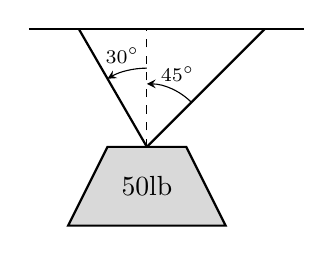
\begin{tikzpicture}
 \filldraw[thick,black,fill=gray!30] (-.5,0) -- (.5,0) -- (1,-1) -- (-1,-1)--cycle;
 \draw (0,-.5) node {50lb};
 \draw [thick] (-1.5,1.5) -- (2,1.5);
 \clip (-1.5,1.5) rectangle (2,-1.25);
 \draw [thick,rotate=120] (0,0) -- (3,0);
 \draw [thick,rotate=45] (0,0) -- (3,0);
 \draw [dashed] (0,0) -- (0,2);
 \draw [rotate=45,->,>=stealth] (.8,0) arc (0:45:.8);
 \draw [rotate=67] (1,0) node {\scriptsize $45^\circ$};
 \draw [rotate=90,->,>=stealth] (1,0) arc (0:30:1);
 \draw [rotate=105] (1.2,0) node {\scriptsize $30^\circ$};
\end{tikzpicture}}{ALT-TEXT-TO-BE-DETERMINED}}

% Example 11.6.2 and several similar examples and exercises need a short physics crash course:  forces are vectors and in particular add like vectors; an object is at rest iff all acting forces add up to the zero vector; force = mass times acceleration; the force of gravity near the surface of the earth is such that the acceleration of every object is 9.8 m/s^2.
\begin{example}[Finding Component Forces]\label{ex_vect6}
Consider a weight of 50lb hanging from two chains, as shown in \autoref{fig:vect6}. One chain makes an angle of $30^\circ$ with the vertical, and the other an angle of $45^\circ$. Find the force applied to each chain.
\solution
Knowing that gravity is pulling the 50lb weight straight down, we can create a vector $\vec F$ to represent this force. 
\[\vec F = 50\bracket{0,-1}=\bracket{0,-50}.\]

We can view each chain as ``pulling'' the weight up, preventing it from falling. We can represent the force from each chain with a vector. Let $\vec F_1$ represent the force from the chain making an angle of $30^\circ$ with the vertical, and let $\vec F_2$ represent the force form the other chain. Convert all angles to be measured from the horizontal (as shown in \autoref{fig:vect6b}), and apply \autoref{idea:unit_vectors}. As we do not yet know the magnitudes of these vectors, (that is the problem at hand), we use $m_1$ and $m_2$ to represent them.
\begin{align*}
\vec F_1 &= m_1\bracket{\cos 120^\circ,\sin120^\circ} \\
\vec F_2 &= m_2\bracket{\cos 45^\circ,\sin45^\circ}
\end{align*}
As the weight is not moving, we know the sum of the forces is $\vec 0$. This gives:
\begin{align*}
\vec F + \vec F_1 + \vec F_2 & = \vec 0\\
\bracket{0,-50}+ m_1\bracket{\cos 120^\circ,\sin120^\circ}+ m_2\bracket{\cos 45^\circ,\sin45^\circ}&=\vec 0
\end{align*}

\mtable{A diagram of the force vectors from \autoref{ex_vect6}.}{fig:vect6b}{\pdftooltip{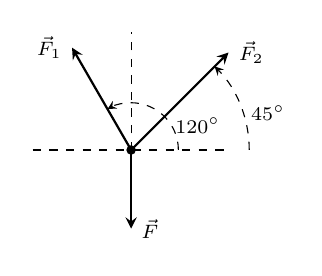
\begin{tikzpicture}[>=stealth]
 \draw [thick,rotate=120,->] (0,0) -- (1.5,0) node [left] {\scriptsize $\vec F_1$};
 \draw [thick,rotate=45,->] (0,0) -- (1.75,0)node [right] {\scriptsize $\vec F_2$};
 \draw [thick,rotate=-90,->] (0,0) -- (1,0) node [right] {\scriptsize $\vec F$};
 \draw [dashed] (0,0) -- (0,1.5);
 \draw [dashed] (-1.25,0) -- (1.25,0);
 \filldraw [black] (0,0) circle (1.5pt);
 \draw [dashed,->,>=stealth] (.6,0) arc (0:120:.6);
 \draw [rotate=20] (.9,0) node {\scriptsize $120^\circ$};
 \draw [dashed,->,>=stealth] (1.5,0) arc (0:45:1.5);
 \draw [rotate=15] (1.8,0) node {\scriptsize $45^\circ$};
\end{tikzpicture}}{ALT-TEXT-TO-BE-DETERMINED}}

The sum of the entries in the first component is 0, and the sum of the entries in the second component is also 0. This leads us to the following two equations:
\begin{align*}
m_1\cos120^\circ + m_2\cos45^\circ &=0 \\
m_1\sin120^\circ + m_2\sin45^\circ &=50
\end{align*}
This is a simple 2-equation, 2-unknown system of linear equations. We leave it to the reader to verify that the solution is 
\[
m_1=50(\sqrt{3}-1)\text{lb}% \approx 36.6
;\qquad
m_2=\frac{50\sqrt{2}}{1+\sqrt{3}}\text{lb}.% \approx 25.88.
\]

It might seem odd that the sum of the forces applied to the chains is more than 50lb. We leave it to a physics class to discuss the full details, but offer this short explanation. Our equations were established so that the \emph{vertical} components of each force sums to 50lb, thus supporting the weight. Since the chains are at an angle, they also pull against each other, creating an ``additional'' horizontal force while holding the weight in place.
\end{example}

Unit vectors were very important in the previous calculation; they allowed us to define a vector in the proper direction but with an unknown magnitude. Our computations were then computed component-wise. Because such calculations are often necessary, the \emph{standard unit vectors} can be useful.

\begin{definition}[Standard Unit Vectors]\label{def:standard_unit}
\index{vectors!standard unit vector}\index{unit vector!standard unit vector}%
\mbox{}\\[-2\baselineskip]\parbox[t]{\linewidth}{\begin{enumerate}
	\item In $\mathbb{R}^2$, the standard unit vectors are
	\[\veci =\bracket{1,0}\quad \text{and}\quad \vecj =\bracket{0,1}.\]
	\item In $\mathbb{R}^3$, the standard unit vectors are
	\[\veci =\bracket{1,0,0}\quad \text{and}\quad \vecj =\bracket{0,1,0}\quad \text{and}\quad \vec k =\bracket{0,0,1}.\]
\end{enumerate}}
\end{definition}

\begin{example}[Using standard unit vectors]\label{ex_vect7}
\mbox{}\\[-2\baselineskip]\parbox[t]{\linewidth}{%
\begin{enumerate}
	\item Rewrite $\vec v =\bracket{2,-3}$ using the standard unit vectors.
	\item	Rewrite $\vec w = 4\veci - 5\vecj +2\vec k$ in component form.
\end{enumerate}}\vspace{0pt}
\solution
\begin{enumerate}
	\item  \hfill$\begin{aligned}[t]
		\vec v &=\bracket{2,-3}\\
		&=\bracket{2,0}+\bracket{0,-3}\\
		&= 2\bracket{1,0}-3\bracket{0,1}\\
		&= 2\veci - 3\vecj
	\end{aligned}$\hfill\null
	
	\item	\hfill$\begin{aligned}[t]
		\vec w &= 4\veci - 5\vecj +2\vec k\\
		&=\bracket{4,0,0}+\bracket{0,-5,0}+\bracket{0,0,2}\\
		&=\bracket{4,-5,2}
	\end{aligned}$\hfill\null
\end{enumerate}
These two examples demonstrate that converting between component form and the standard unit vectors is rather straightforward. Many mathematicians prefer component form, and it is the preferred notation in this text. Many engineers prefer using the standard unit vectors, and many engineering texts use that notation.
\end{example}

\begin{example}[Finding Component Force]\label{ex_vect8}
A
%
\mtable{A figure of a weight being pushed by the wind in \autoref{ex_vect8}.}{fig:vect8}{\pdftooltip{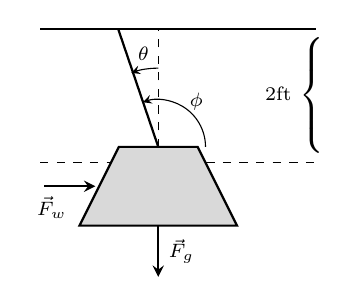
\begin{tikzpicture}
 \draw [dashed] (-1.5,-.2) -- (2,-.2);
 \draw (1.75,.65) node {\scriptsize 2ft $\left\{\rule{0pt}{.8cm}\right.$};
 \filldraw[thick,black,fill=gray!30] (-.5,0) -- (.5,0) -- (1,-1) -- (-1,-1)--cycle;
 \draw [thick] (-1.5,1.5) -- (2,1.5);
 \draw [thick] (0,0) -- (-.51,1.5); % diagonal line ~ 110 degrees
 \draw [dashed] (0,0) -- (0,1.5);
 \draw [rotate=90,->,>=stealth] (1,0) arc (0:20:1);
 %
 \draw [->,>=stealth] (.6,0) arc (0:109:.6);
 \draw [rotate=50] (.75,0) node {\scriptsize $\phi$};
 %
 \draw [rotate=99] (1.2,0) node {\scriptsize $\theta$};
 \draw [thick,->,>=stealth] (-1.45,-.5) -- (-.8,-.5) node [pos=.15,below] {\scriptsize $\vec F_w$};
 \draw [thick,->,>=stealth] (0,-1) -- (0,-1.65) node [pos=.5,right] {\scriptsize $\vec F_g$};
\end{tikzpicture}}{ALT-TEXT-TO-BE-DETERMINED}}
%
weight of 25lb is suspended from a chain of length 2ft while a wind pushes the weight to the right with constant force of 5lb as shown in \autoref{fig:vect8}. What angle will the chain make with the vertical as a result of the wind's pushing? How much higher will the weight be?
\solution
The force of the wind is represented by the vector $\vec F_w = 5\veci$. The force of gravity on the weight is represented by $\vec F_g = -25\vecj$. The direction and magnitude of the vector representing the force on the chain are both unknown. We represent this force with
\[\vec F_c = m\bracket{\cos\phi,\sin\phi}= m\cos\phi\, \veci + m\sin\phi\,\vecj\]
for some magnitude $m$ and some angle with the horizontal $\phi$. (Note: $\theta$ is the angle the chain makes with the \emph{vertical}; $\phi$ is the angle with the \emph{horizontal}.)

As the weight is at equilibrium, the sum of the forces is $\vec0$:
\begin{align*}
\vec F_c + \vec F_w + \vec F_g &= \vec 0\\
m\cos\phi\, \veci + m\sin\phi\,\vecj + 5\veci - 25\vecj &=\vec 0
\end{align*}

Thus the sum of the $\veci$ and $\vecj$ components are 0, leading us to the following system of equations:
\begin{align}
5+m\cos\phi &= 0\\
-25+m\sin\phi &= 0
\label{eq:vect8}
\end{align}

This is enough to determine $\vec F_c$ already, as we know $m\cos \phi = -5$ and $m\sin\phi =25$. Thus $F_c =\bracket{-5,25}.$ We can use this to find the magnitude $m$:
\[m = \sqrt{(-5)^2+25^2} = 5\sqrt{26}%\approx 25.5
\text{lb}.\]
We can then use either equality from \autoeqref{eq:vect8} to solve for $\phi$. We choose the first equality as using arccosine will return an angle in the $2^\text{nd}$ quadrant:
\[5 + 5\sqrt{26}\cos \phi = 0 \quad \Rightarrow \quad \phi = \cos^{-1}\left(\frac{-5}{5\sqrt{26}}\right) \approx 1.7682\approx 101.31^\circ.\]

Subtracting $90^\circ$ from this angle gives us an angle of $11.31^\circ$ with the vertical.

We can now use trigonometry to find out how high the weight is lifted. \autoref{fig:vect8} shows that a right triangle is formed with the 2ft chain as the hypotenuse.  We have found that the interior angle is $11.31^\circ$. The length of the adjacent side (in the diagram, the dashed vertical line) is $2\cos 11.31^\circ \approx 1.96$ft. Thus the weight is lifted by about $0.04$ft, almost 1/2in.
\end{example}

The algebra we have applied to vectors is already demonstrating itself to be very useful. There are two more fundamental operations we can perform with vectors, the \emph{dot product} and the \emph{cross product}. The next two sections explore each in turn.

\printexercises{exercises/10-02-exercises}
